\documentclass[output=paper,colorlinks,citecolor=brown,
% hidelinks,
% showindex
]{langscibook}
\author{Chiyo Nishida\affiliation{University of Texas-Austin} and Cinzia Russi\affiliation{University of Texas-Austin}}
\title{Italian and Spanish unaccusative sentence focus constructions: What corpora tell us about
their word order}
\abstract{Traditionally, VS has been argued to be the canonical word order for Italian and Spanish unaccusative sentences instantiating \textsc{sentence focus} (SF). However, corpus data show that SV order extensively occurs in SF contexts. Through a quantitative and a qualitative analysis of corpus data this study demonstrates that the two word orders represent two constructions each fulfilling a distinct discourse function. The quantitative analysis examined a total of 1,670 tokens of VS and SV sentences with the verbs \textit{arrivare/llegar} `to arrive' and \textit{morire/morir} `to die' with respect to several linguistic and extralinguistic factors. The statistical results revealed that, for both languages, the most decisive factor distinguishing SV from VS sentences was the distribution of adverbials: while the odds of occurrence of SV sentences significantly decrease (p<.0001) with the presence of clause-initial adverbials, they significantly increase (p<.0001) with the presence of postverbal adverbials. The qualitative analysis looked closely at the highly concentrated preverbal adverbials in VS sentences and postverbal adverbials in SV sentences using a data set that included two additional verbs, \textit{cadere/caer} `to fall' and \textit{comparire/aparecer} `to appear'. We found that the preverbal adverbials in VS sentences are most typically presupposed spatio-temporal elements; the postverbal adverbials in SV sentences constituted a diverse mix of elements. From these findings, we conclude that VS unaccusative sentences present a new event highlighting the (dis)appearance of the subject referent and framed by a topical element. SV sentences likewise depict a new event but in elaboration of its circumstantial details and without being framed by any topical element.
}
  
\setlength{\footheight}{32.53401pt} 

\IfFileExists{../localcommands.tex}{
  \addbibresource{localbibliography.bib}
  % add all extra packages you need to load to this file

\usepackage{tabularx,multicol,multirow}
\usepackage{url}
\urlstyle{same}

\usepackage{listings}
\lstset{basicstyle=\ttfamily,tabsize=2,breaklines=true}

\usepackage{langsci-basic}
\usepackage{langsci-optional}
\usepackage{langsci-lgr}
\usepackage{langsci-gb4e}
%    \let\eachwordone=\it % Ch 14, 18

\usepackage{jambox}
\usepackage{subfigure}
\usepackage{tablefootnote}
\usepackage[nameinlink, noabbrev]{cleveref}
\crefname{enumi}{example}{examples}

\usepackage{bbding}
%\usepackage{linguex}
\usepackage{stmaryrd}

\usepackage{tipa}
\let\ipa\textipa
\usepackage{vowel}
\newcommand{\BlankCell}{}
\usepackage{ot-tableau}

\usepackage{forest}
\useforestlibrary{linguistics}
\usepackage[noeepic]{qtree}
\usepackage{pstricks, pst-xkey, pst-jtree}
\usepackage{tikz-qtree}
\usepackage{tikz-qtree-compat}
\usepackage{tree-dvips}

\usepackage{lastpage}
\usepackage{hyperref}
\usepackage{xltxtra}

\usepackage{ragged2e}
%\usepackage{subcaption}
\usepackage{floatrow}
\usepackage{float}

\usepackage[normalem]{ulem} % Pour les textes barrés
\usepackage{ifthen} 

\usepackage{todonotes}

  \newcommand*{\orcid}{}

\makeatletter
\let\theauthor\@author
\makeatother

\papernote{\scriptsize\normalfont
    \theauthor.
    \titleTemp. 
    To appear in: 
    Chad Howe and Pilar Chamorro and Timothy Gupton and Margaret Renwick.
    Theory, Data, and Practice: Selected papers from the 49th Linguistic Symposium on Romance Language
    Berlin: Language Science Press. [preliminary page numbering]
}

% Workaround for subscripts with capital letters
\newcommand{\capsub}[1]{\ensuremath{_\text{#1}}}

% Chapter 10: Table-like presentation within example environment
% classical latin > {*}late latin > old french  earlier > later   gloss
\newcommand{\montanoboxi}[7]{\parbox{2cm}{#1} > {#2}\parbox{2cm}{#3} > \parbox{1.5cm}{\textit{#4}} \parbox{1.2cm}{#5}\ > \parbox{1.2cm}{#6} \parbox{1.5cm}{#7}}
% {*}latin > earlier OF [ipa] > early OF   gloss
\newcommand{\montanoboxii}[6]{{#1}\parbox{1.9cm}{\textit{#2}} > \parbox{1.3cm}{\textit{#3}} \parbox{2cm}{#4} \parbox{2cm}{#5} \parbox{1.9cm}{#6}}

% Chapter 5
\newcommand{\redc}[1]{\textcolor{red}{#1}}
\newcommand{\bluec}[1]{\textcolor{blue}{#1}}
\newcommand{\ajout}[1]{\textcolor{blue}{#1}}
\newcommand{\ajoutplus}[1]{\textcolor{cyan}{#1}}

\newcommand{\hachure}[9]{
% Parametres :
% Coordonnees bas gauche (2 parametres) : (#1,#2)
% Coordonnees haut droit (2 parametres) : (#3,#4)
% Orientation : #5
%   1 : diagonale de pente 1
%  -1 : diagonale de pente -1
%   0 : horizontal
%   2 : vertical
% Nombre de pas horizontaux : #6
% Epaisseur du trait : #7
% Couleur : #8 (ex. green)
% Atténuation couleur : #9 (ex. 30)
\pgfmathsetmacro{\N}{#6-1}
\pgfmathsetmacro{\A}{#1}
\pgfmathsetmacro{\B}{#2}
\pgfmathsetmacro{\C}{#3}
\pgfmathsetmacro{\D}{#4}
\pgfmathsetmacro{\I}{(#3-#1)/#6}
\pgfmathsetmacro{\J}{(#4-#2)/#6}
\ifthenelse{\equal{#5}{1}}{
  \foreach \n in {0,...,\N}
    \foreach \m in {0,...,\N}
      {
        \pgfmathsetmacro{\X}{\A + ((0 + \n) * \I)}
        \pgfmathsetmacro{\Y}{\B + ((0 + \m) * \J)}
        \pgfmathsetmacro{\U}{\A + ((1 + \n) * \I)}
        \pgfmathsetmacro{\V}{\B + ((1 + \m) * \J)}
        \draw[#8!#9,#7] (\X, \Y)--(\U, \V);
      } 
  }{}
\ifthenelse{\equal{#5}{-1}}{
  \foreach \n in {0,...,\N}
    \foreach \m in {0,...,\N}
      {
        \pgfmathsetmacro{\X}{\A + ((1 + \n) * \I)}
        \pgfmathsetmacro{\Y}{\B + ((0 + \m) * \J)}
        \pgfmathsetmacro{\U}{\A + ((0 + \n) * \I)}
        \pgfmathsetmacro{\V}{\B + ((1 + \m) * \J)}
        \draw[#8!#9,#7] (\X, \Y)--(\U, \V);
      } 
  }{}
\ifthenelse{\equal{#5}{0}}{
  \foreach \n in {0,...,\N}
    \foreach \m in {0,...,\N}
      {
        \pgfmathsetmacro{\X}{\A + ((0 + \n) * \I)}
        \pgfmathsetmacro{\Y}{\B + ((0 + \m) * \J)}
        \pgfmathsetmacro{\U}{\A + ((1 + \n) * \I)}
        \pgfmathsetmacro{\V}{\B + ((0 + \m) * \J)}
        \draw[#8!#9,#7] (\X, \Y)--(\U, \V);
      } 
  }{}
\ifthenelse{\equal{#5}{2}}{
  \foreach \n in {0,...,\N}
    \foreach \m in {0,...,\N}
      {
        \pgfmathsetmacro{\X}{\A + ((0 + \n) * \I)}
        \pgfmathsetmacro{\Y}{\B + ((0 + \m) * \J)}
        \pgfmathsetmacro{\U}{\A + ((0 + \n) * \I)}
        \pgfmathsetmacro{\V}{\B + ((1 + \m) * \J)}
        \draw[#8!#9,#7] (\X, \Y)--(\U, \V);
      } 
  }{}
}

%Définition d'un pattern de type hachure
% \usetikzlibrary{patterns}
% \makeatletter
% \tikzset{hatch distance/.store in=\hatchdistance,hatch distance=5pt,hatch thickness/.store in=\hatchthickness,hatch thickness=5pt}

% \pgfdeclarepatternformonly[\hatchdistance,\hatchthickness]{north east hatch}% name
%     {\pgfqpoint{-\hatchthickness}{-\hatchthickness}}% below left
%     {\pgfqpoint{\hatchdistance+\hatchthickness}{\hatchdistance+\hatchthickness}}% above right
%     {\pgfpoint{\hatchdistance}{\hatchdistance}}%
%     {
%         \pgfsetcolor{\tikz@pattern@color}
%         \pgfsetlinewidth{\hatchthickness}
%         \pgfpathmoveto{\pgfqpoint{-\hatchthickness}{-\hatchthickness}}       
%         \pgfpathlineto{\pgfqpoint{\hatchdistance+\hatchthickness}{\hatchdistance+\hatchthickness}}
%         \pgfusepath{stroke}
%     }
% \pgfdeclarepatternformonly[\hatchdistance,\hatchthickness]{north west hatch}% name
%     {\pgfqpoint{-\hatchthickness}{-\hatchthickness}}% below left
%     {\pgfqpoint{\hatchdistance+\hatchthickness}{\hatchdistance+\hatchthickness}}% above right
%     {\pgfpoint{\hatchdistance}{\hatchdistance}}%
%     {
%         \pgfsetcolor{\tikz@pattern@color}
%         \pgfsetlinewidth{\hatchthickness}
%         \pgfpathmoveto{\pgfqpoint{\hatchdistance+\hatchthickness}{-\hatchthickness}}
%         \pgfpathlineto{\pgfqpoint{-\hatchthickness}{\hatchdistance+\hatchthickness}}
%         \pgfusepath{stroke}
%     }
% \makeatother
%~~~~~~~~~~~~~~~~~~~~~~~~~~~~~~~~~~~~~


% Chapter 7
\newcommand\pef[1]{(\ref{#1})}

\newcommand{\subscript}[1]{\textsubscript}
 
  %% hyphenation points for line breaks
%% Normally, automatic hyphenation in LaTeX is very good
%% If a word is mis-hyphenated, add it to this file
%%
%% add information to TeX file before \begin{document} with:
%% %% hyphenation points for line breaks
%% Normally, automatic hyphenation in LaTeX is very good
%% If a word is mis-hyphenated, add it to this file
%%
%% add information to TeX file before \begin{document} with:
%% %% hyphenation points for line breaks
%% Normally, automatic hyphenation in LaTeX is very good
%% If a word is mis-hyphenated, add it to this file
%%
%% add information to TeX file before \begin{document} with:
%% \include{localhyphenation}
\hyphenation{
anaph-o-ra
Dor-drecht
%FFI2016-76045-P-AEI/-MINEICO/-FEDE
}

\hyphenation{
anaph-o-ra
Dor-drecht
%FFI2016-76045-P-AEI/-MINEICO/-FEDE
}

\hyphenation{
anaph-o-ra
Dor-drecht
%FFI2016-76045-P-AEI/-MINEICO/-FEDE
}
 
  \togglepaper[23]%%chapternumber
}{}

\begin{document}
\maketitle

\section{Introduction}\label{sec:nishida:1}

Traditionally, VS has been argued to be the canonical word order for Italian and Spanish unaccusative sentences instantiating \textsc{sentence focus} (SF), \textit{aka}
\textsc{broad/}
\textsc{wide} or \textsc{neutral focus} (\citealt{contreras1976theory}; \citealt{lambrecht1994}; \citeyear{lambrecht2000subjects}, \citealt{gutierrez2007prominence}; \textit{inter alia}).\footnote{VS is also the order for instantiating \textsc{argument} (subject) focus.} \citet[612]{lambrecht2000subjects} defines \textsc{focus} as ``the element of a pragmatically structured proposition whose occurrence makes it possible for the sentence to express a `pragmatic assertion', i.e., to convey new information to an addressee'' (cf. also \citealt[27]{erteschik1999focus}'s definition of focus as ``the nonpresupposed information in the sentence'')\footnote{Following  \citet[74]{jackendoff1972}, focus is commonly defined  as the element providing 
``a resolution for a variable left open in previous discourse''; for instance, wh-questions like \textit{What did John study?} involve a piece of information unspecified, as represented by the variable x in [x|John studied].  In the response sentence \textit{John studied music}, focus is the part that provides a resolution to the variable \textit{x: music} (cf. also  \citealt{zubizarreta1998},  \citealt{lopez2009derivational}; \textit{inter alia}.}, and SF as 
``the domain of `new information' that extends over the entire proposition'' \citep[14]{lambrecht1994}, the proposition being ``the subject and the predicate (minus any topical non-subject elements)'' \citep[222]{lambrecht1994}. Following this definition, the bracketed VS strings in the corpus passages in \ref{ex:nishida:1} below constitute SF, supporting the traditional analysis.\footnote{The data in this paper come from two online corpora: \textit{Corpus di italiano scritto} (CORIS/CODIS) for Italian and \textit{Corpus de Referencia del Español Actual} (CREA) for Spanish. CORIS/CODIS consists of 130 million words and comprises authentic and commonly occurring texts considered highly representative of modern Italian from an assortment of diverse genres (press, fiction, academic, legal and administrative prose, miscellanea). CREA, compiled by the Spanish Royal Academy, amounts to 200 million words and stores samples from 1974 to 2004, classified according to genre (press, books, miscellaneous, and oral), field (Science \& Technology, Social Sciences, Arts, Entertainment, Health, Fiction, etc.) and country (Spain, Hispanic American countries, Philippines, and the US). We considered only written data from European Spanish. For both languages all passages are noted only for genres.  Throughout the paper the source language in the examples is abbreviated as It. for Italian and Sp. for Spanish.} 

\begin{exe} % declares the example environment
    \ex\label{ex:nishida:1}
    \begin{xlist} % declares a list of sub-examples
        \ex\label{ex:nishida:1a} Dalla strage del 12 aprile sul treno della Val Venosta, in Alto Adige, emergono documenti 
	inquietanti. Nell’incidente [\capsub{FOC} \textbf{sono morte nove persone}], una ventina i feriti. (It.; press)
	\glt 	‘From the April 12 massacre on board the Val Venosta train, in Alto Adige, emerge 	disturbing documents. In the incident [\capsub{FOC} \textbf{nine people died}], about twenty casualties.’
        \ex\label{ex:nishida:1b} Un compañero del Partido le dijo que después trasladaron un gran número de mujeres a 
	Madrid. Las llevaron en tren. En el trayecto [\capsub{FOC} \textbf{murieron cinco niños}.] (Sp.; fiction)
	\glt ‘A buddy from the Party told him that afterwards they transported a great number of women 	to Madrid. They took them by train. On the journey [\capsub{FOC} \textbf{ five children died}].’ 
\end{xlist}
\end{exe}

However, data from corpora reveal that SV order occurs extensively in SF contexts in both Italian and Spanish, as illustrated in \ref{ex:nishida:2}.


\begin{exe} % declares the example environment
    \ex\label{ex:nishida:2} 
    \begin{xlist} 
        \ex\label{ex:nishida:2a} “L’acqua non è una merce.” Ripetetelo allo specchio ogni mattina: vi darà consapevolezza. I numeri parlano chiaro e ci sussurrano dati che non vogliamo 	ascoltare. Un miliardo di persone non ha acqua potabile. [\capsub{FOC} \textbf{Un milione ottocentomila 			bambini muoiono} ogni anno per malattie causate dall’acqua inquinata]. (It.; press)
        \glt ```Water is not merchandise." Repeat it every morning while looking at yourself in the 			mirror. The numbers speak clearly and whisper to us data that we don’t want to hear. One 		billion people do not have drinking water. [\capsub{FOC} \textbf{One million eight hundred thousand 				children} die every year from diseases caused by polluted water].'	
        \ex\label{ex:nishida:2b} En el parte de noticias el locutor dijo: [\capsub{FOC} “\textbf{Mujeres y niños mueren de manera					indescriptiblemente dolorosa en Chipre}.”] (Sp.; fiction)
        \glt ‘In the news report the caster said: [\capsub{FOC} “\textbf{Women and children die in a manner 					indescribably painful in Cyprus}.”]’   
          
\end{xlist}
\end{exe}


The bracketed SV sentences in \ref{ex:nishida:2} constitute new information in their entirety; neither the subject nor the predicate in these sentences is part of pragmatic presupposition and known to the reader. Therefore, any other alternative focus structure (i.e., predicate focus or (preposed) contrastive argument focus) cannot be assigned to these sentences.\footnote{Contrastive focus is ruled out since the sentences in \ref{ex:nishida:2} do not convey information that is contrary to/contrasts with the addressee's presuppositions, as is evident from the context.}

In view of the data in \ref{ex:nishida:1} and \ref{ex:nishida:2}, a natural question arises: If both VS and SV unaccusative sentences may instantiate SF, are the two constructions free variants that can be used interchangeably in the same discourse context? Or do they fulfill distinct functions? 


That both VS and SV order may instantiate SF has been previously noted by \citet{pinto1997} for Italian and others who have embraced her account (cf. \citeauthor{Sheehan2006} \citeyear{Sheehan2006}, \citeyear{Sheehan2010}; \citeauthor{corr2016wide} \citeyear{corr2016wide}; \textit{inter alia}). Although these studies offer valuable insights, they are purely syntactic in nature and are not concerned with how the two constructions may differ in the way they are used in discourse contexts.  

This paper presents the results of a corpus study showing that the two SF constructions with unaccusatives are not free variants and proposes that each assumes a distinct function in discourse contexts. After a brief review of some relevant literature on the topic in \ref{sec:nishida:2}, in \ref{sec:nishida:3}--\ref{sec:nishida:4} we present our corpus study in two parts. First (\ref{sec:nishida:3}), through a quantitative analysis of VS and SV unaccusative sentences gathered from online corpora, we show that the property that most crucially distinguishes the SV construction from its VS counterpart is the distribution of co-occurring adverbials: while the presence of clause-initial adverbials significantly decreases the odds of occurrence of the SV construction, the presence of postverbal adverbials increases such odds. Second (\ref{sec:nishida:4}), we report on a qualitative analysis that primarily compares postverbal adverbials occurring in the SV construction with highly concentrated preverbal adverbials in the VS construction and identify another key distinguishing property: while clause-initial adverbials in the VS construction are restricted to topical XPs (the most common of which are spatio-temporal elements), postverbal adverbials in the SV construction consist of a non-topical, diverse mix of circumstantial elements. Based on these findings we delineate the two distinct functions assumed by the two SF constructions: (a) the VS construction presents a new event highlighting the (dis)appearance of the subject referent typically framed by a topical spatio-temporal element; (b) the SV construction depicts a new event with an elaboration of how it transpires as part of focus and without being framed by a topical element.  
Therefore, the commonly proposed characterization of VS unaccusative sentences as an answer to the question ``What happened?'' or as a discourse-initial ``out-of-the-blue'' statement turns out to be inaccurate. Such a characterization, in fact, appears to be more suited for SV sentences. In \ref{sec:nishida:5} we conclude by summarizing the study.


\section{VS and SV sentence focus constructions: a brief review}\label{sec:nishida:2}

Romance VS intransitive sentences of the type shown in \ref{ex:nishida:1} above have been a fertile area of research from different perspectives and have produced a great number of studies. However, here we must limit ourselves to review only a handful. Before formal syntacticians started working on VS unaccusative sentences within relational and generative grammar (cf. \citealt{perlmutter1978,burzio1986italian}; \textit{inter alia}), it is noteworthy that these sentences had been characterized as \textsc{presentational sentences} by \citet{hatcher1956}. Later, \citet{suner1982}, largely following Hatcher, claims that a Spanish VS intransitive sentence like \textit{Apareció Paco} `There/here appeared Paco'  
``carries existential assertion: it asserts that the object exists in the universe of discourse'' \citep[126]{suner1982}. The group of verbs that Hatcher and Suñer define as presentational in Spanish largely overlaps with unaccusatives, though they are not referenced as such at the time. Presentational sentences in Romance languages are assimilated to the construction known as \textsc{locative inversion} (e.g., \citealt{tortora1997,cornish2005cross,ortega2005locative,Sheehan2006,lahousse2007implicit,teixeira2016locative,bentley2018silent} (B\&C, hereafter); \textit{inter alia}) or subject inversion (e.g., \citealt{marandin2010subject}), which is known to exist in many languages of the world, the most widely examined one being English (e.g., \textit{Over the mountains appeared dark clouds}; cf. \citealt{birner1994information,levinrap1995}; \textit{inter alia}). 

In his typological work, which includes French, Italian, and European Portuguese, \citet[2, our emphasis]{cornish2005cross} proposes that the discourse function of inversion sentences is ``to present a referent which is discourse new \textit{within the framework of locative or temporal context}''. Erteschik-Shir (\citeyear{erteschik1997dynamics,erteschik1999focus}) labels the element providing such a spatio-temporal framework \textsc{stage topic} (s\textsc{top}) and defines it as 
``the spatio-temporal parameters of the utterance. Stage topics may be overt (`this afternoon', `on Park Avenue'), or discursively implied (the here-and-now)'' \citep[124]{erteschik1999focus}, where the term stage denotes ``the Time/Place at which the event expressed by the sentence takes place'' \citep[26--27]{erteschik1997dynamics}. According to Erteschik-Shir, the s\textsc{top} is just like a regular topic; hence, its referent must be identifiable (i.e., pragmatically presupposed) by the speaker and the hearer. \citet[2]{lahousse2007implicit} refines the function of the s\textsc{top} further citing \citet[50]{chafe1976givenness}: 
``The topic sets a spatial, temporal, or individual framework within which the main predication holds''. 

Going back to the VS sentences in \ref{ex:nishida:1}, the preverbal PPs both qualify as s\textsc{top}s because (a) they provide the spatio-temporal framework within which events introducing the subject referents take place; and (b) they are pragmatically presupposed XPs because they are anaphorically retrievable from the previous mention of the ``April 12$^{th}$ train massacre'' and the ``transfer of women to Madrid by train'' in the discourse. 

Working on French data, \citet{lahousse2007implicit} claims that it is in fact a s\textsc{top} that licenses the subject to appear postverbally. However, VS sentences in Romance languages may lack an explicit s\textsc{top} in the preverbal position, as shown in the bracketed sentence in the passage in \ref{ex:nishida:3}, which is an instance of what Lahousse calls \textsc{absolute inversion}.

\begin{exe} % declares the example environment
    \ex\label{ex:nishida:3} 
   Entro le 14 bisogna abbandonare Valona. [$\emptyset$ \textbf{Arrivano auto dei rivoltosi}]: 
   si offrono di 	trasportare i giornalisti in un vecchio aeroporto militare dismesso al centro della città dove pare che atterrerà l’elicottero italiano. (It.; press)
   \glt ‘By 2pm Valona must be abandoned. [\textbf{Here/There arrive cars with rebels}]: it is offered to 	transport the journalists to an old abandoned military airport in the center of the city where 	the Italian helicopter is expected to land.’ 
\end{exe}

Following Erteschik-Shir's work, \citet{lahousse2007implicit} and \citet{teixeira2016locative} argue that an absolute inversion sentence has a covert s\textsc{top} that, like an overt s\textsc{top}, licenses subject-verb inversion.\footnote{Syntactically, the PP serving as a s\textsc{top} (overt or covert) is argued by some to occupy the specifier position of TP to satisfy EPP (cf. 
\citealt{pinto1997}; \citealt{ortega2005locative}; \citealt{Sheehan2006}, \citeyear{Sheehan2010}; \textit{inter alia}).}
Texeira identifies two types of covert s\textsc{top}: one is interpreted deictically (i.e., here and now) and the other anaphorically (i.e., then and there). The bracketed sentence in \ref{ex:nishida:3} is indeed interpreted with the spatio-temporal framework ``at 2pm \& in Valona'', mentioned in the previous sentence.\footnote{We do not postulate that such an interpretation arises on account of a covert element occupying the preverbal position; rather, we propose that it arises because the reader thinks that is the felicitous interpretation judging from the context.}

B\&C (\citeyear[2]{bentley2018silent}) address the licensing of subject inversion in broad focus constructions which lack overt sentence-initial spatio-temporal phrases, and argue that subject inversion is licensed by a ``silent preverbal argument'' which they call \textsc{Subject of Predication} (SoP). Specifically, they identify two subtypes of SoP; the first is ``a thematic argument selected by the verb'' B\&C \citeyear[2]{bentley2018silent}, such as the locative goal of verbs of motion discussed by \citet{tortora1997}, exemplified by \textit{Sono arrivati gli studenti} 
`The students have arrived (here)', or the benefactive goal argument in \textit{Hanno telefonato i ragazzi} `The kids have phoned (here/us)'. The second type of SoP, is ``a non-thematic situational argument'' which is not provided by previous context or co-text; rather, it is ``inferred when there is no thematic goal available to provide the SoP'' B\&C \citeyear{bentley2018silent}, exemplified by \textit{Sono morti i soldati} 
`The soldiers have died'.

As has been pointed out (e.g., \citealt{torrego1989}; \citealt{pinto1997}; B\&C \citeyear{bentley2018silent}; \textit{inter alia}), subject inversion also extends to unergatives, as shown in corpus data in \ref{ex:nishida:4} and \ref{ex:nishida:5}.


\begin{exe} % declares the example environment
    \ex\label{ex:nishida:4} 
    \begin{xlist} 
        \ex\label{ex:nishida:4a} In quest’area a vocazione agricola – estremo lembo della Lombardia al confine con 		Veneto ed Emilia – \textbf{abitano} circa 30 mila persone. (It.; press)
         \glt ‘In this area devoted to agriculture – the extreme strip of Lombardia bordering 	eneto and Emilia – live about 30 thousand people.’
        \ex\label{ex:nishida:4b} {\dots} de hecho en Jerusalén Este \textbf{viven} 150.000 palestinos y en Cisjordania \textbf{habitan} cerca de 140.000 israelíes. (Sp.; press)
         \glt ‘{\dots}  in fact in East Jerusalem live 150,000 Palestinians and in Cisjordan live close to 				140,000 Israelis.’  
\end{xlist}
\end{exe}


\begin{exe} % declares the example environment
    \ex\label{ex:nishida:5} 
    \begin{xlist} 
        \ex\label{ex:nishida:5a} Al progetto per la riforma del linguaggio burocratico \textbf{lavorano} 10 persone, fra giuristi e 			linguisti. (It.; press)
        \glt ‘On the project for the reform of bureaucratic language are working ten people, jurists and linguists among them.’ 
          
        \ex\label{ex:nishida:5b} En el zoo \textbf{trabajan} veinte personas más que se ocupan de muy variadas tareas. (Sp.; non-fiction) 
        \glt ‘At the zoo are working twenty more persons that are occupied with very varied tasks.’ 
          
\end{xlist}
\end{exe}


However, VS sentences with unergative verbs show properties that are very different from their unaccusative counterparts in that they are far more constrained. As \citet{torrego1989} and \citet{pinto1997} pointed out, the preverbal XP for VS unergative sentences are restricted mostly to locative phrases. Moreover, unlike their unaccusative counterparts, unergative VS sentences would be ungrammatical without an overt preverbal phrase.\footnote{There are a few unergatives that can occur in VS order and without a preverbal XP. One such verb is \textit{telefonare/llamar} `to phone'. See \citet{corr2016wide} and B\&C (\citeyear{bentley2018silent}) for detailed discussions.} Also, a quick corpus search indicates that they tend to occur more with imperfective tenses like present, as in \ref{ex:nishida:4} and \ref{ex:nishida:5} above, or the imperfect indicative than with perfective tenses. This grammatical aspect bias may be related to the lexical aspectual property of unergative verbs of being atelic.

We now turn our attention to SV unaccusative sentences instantiating SF. These sentences have received very little attention in past research compared to their VS counterparts, although they have been acknowledged to exist. For instance, \citet{pinto1997} observes that in Italian both VS and SV sentences may be used with certain intransitive verbs to mark broad focus (our SF), as contrasted in \ref{ex:nishida:6} and \ref{ex:nishida:7} below (cf. also \citealt{antinucci1977sull}; \citealt{sornicola1994}). \citet{corr2016wide}
makes similar observations for different varieties of Spanish.



\begin{exe} % declares the example environment
    \ex\label{ex:nishida:6} 
    \begin{xlist} 
        \ex\label{ex:nishida:6a} È entrato Dante.\jambox{VS}
        \glt ‘Dante entered (here/into this place).’
          
        \ex\label{ex:nishida:6b} Dante è entrato.\jambox{SV}
        \glt ‘Dante entered (into some place).’ \citep[188, ex. 19a-b]{pinto1997} 
\end{xlist}
\end{exe}

\begin{exe} % declares the example environment
    \ex\label{ex:nishida:7} 
    \begin{xlist} 
        \ex\label{ex:nishida:7a} È morto Fellini.\jambox{VS}
        \glt ‘Fellini has (just) died.’ (I just heard that F. died)
          
        \ex\label{ex:nishida:7b} Fellini è morto.\jambox{SV}
        \glt ‘Fellini died (sometime).’ \citep[118,~exx.~20a--b]{pinto1997}
          
\end{xlist}
\end{exe}

Pinto claims that VS and SV sentences differ semantically, as annotated in the translation. She explains that while VS sentences obligatorily receive a `deictic' (defined as `speaker-oriented') loco (=spatio)-temporal interpretation, SV sentences are not linked exclusively to this interpretation. She goes on to explain how VS sentences like \ref{ex:nishida:6a} and \ref{ex:nishida:7a}, which lack an explicit preverbal XP, are derived, and then proposes that the group of verbs she calls \textsc{broad focus inversion verbs} – which largely overlap with unaccusatives like \textit{entrare} 
`to enter' and \textit{morire} `to die' – select an extra internal loco-temporal argument (\textsc{loc}). This argument can either be overt or covert, but it must be deictic. Thus, in order to derive VS sentences like \ref{ex:nishida:6a} and \ref{ex:nishida:7a}, a covert subcategorized deictic \textsc{loc} argument is generated inside VP and then moved to the specifier position of TP to satisfy EPP. Clearly, Pinto's proposal stems from an assumption similar to Lahousse's and Texeira's that VS sentences must have a s\textsc{top} in the preverbal position (overt or covert), except that Pinto proposes a formal account of the mechanism through which this element is syntactically integrated into VS sentences.\footnote{Curiously, Pinto does not address VS sentences with unaccusatives accompanied by an overt loco-temporal argument like those shown in \ref{ex:nishida:1}, although these are far more commonly found in corpora than sentences like \ref{ex:nishida:3}. The types of VS sentences with an overt loco-temporal argument she considers only include unergatives (`to live', `to work', `to study', etc.), as exemplified in \ref{ex:nishida:4}--\ref{ex:nishida:5}, for which an overt loco-temporal argument is obligatory.}

Although Pinto's work casts more light on SV sentences than does Lahousse's or Texeira's, it is primarily concerned with the syntactic derivation of VS sentences with a covert \textsc{loc} within the minimalist framework (cf. \citealt{chomsky1995minimalist}); she does not pursue the question as to how the said semantic difference between the VS and SV constructions translates into the different roles the two constructions may play in discourse contexts. Sheehan (\citeyear{Sheehan2006}, \citeyear{Sheehan2010}) and Corr (\citeyear{corr2016wide}), who follow up on Pinto, also focus exclusively on the syntactic derivation of VS sentences with a covert loco-temporal PP, though they use a more recent version of the Minimalist Theory.
Clearly, in order to elucidate how VS and SV sentences are used differently in discourse contexts, it is crucial to examine naturally-occurring data in which the two constructions appear within passages, as shown in \ref{ex:nishida:1} and \ref{ex:nishida:2}, rather than de-contextualized. As we embark on our study, we wish to clarify that we will not consider sentences with unergatives as shown in \ref{ex:nishida:3} and \ref{ex:nishida:4}. Those will have to wait for another study.  

\section{Corpus study part I: quantitative analysis}\label{sec:nishida:3}

The goal of this part of our study is not only to provide empirical evidence that SV sentences are not in free variation with VS sentences but also to identify through a quantitative analysis the properties that significantly distinguish the SV construction from their VS counterpart. 

\subsection{Dataset and analysis}

Using two pairs of verbs \textit{arrivare/llegar} `to arrive' and \textit{morire/morir} `to die', a total of 671 tokens of SV sentences (203 Italian/468 Spanish) and a total of 999 tokens of VS sentences (430 Italian/569 Spanish), all instantiating SF, were extracted from two online corpora (see fn. 1). We retrieved manually all tokens of \textit{arrivare/llegar} and \textit{morire/morir} in the present and perfective (simple and compound) tenses of the indicative mood, occurring in the context of root, coordinate, and subordinate (complement, adverbial relative, and temporal) clauses.\footnote{By `adverbial relative clauses' we mean strings like \textit{la calle en la que suceden muchos accidentes} `the street on which a lot of accidents occur'. See fn.12 below. Temporal clauses included those introduced by \textit{quando/cuando} `when' and \textit{mentre/mientras} `while'.} These two pairs of verbs were selected since a pilot study showed that they occur far more frequently in SV sentences in the corpora than any other unaccusatives. Moreover, we only considered plural subjects because our pilot study had identified quantity specification as a critical distinguishing property of SV order for Spanish. \tabref{tab:nishida:1} summarizes our dataset for the quantitative analysis.

\newpage
\begin{table}
    \begin{tabularx}{\textwidth}{lrlrllrlr}
    \lsptoprule
         &  \multicolumn{3}{c}{SV} & & &  \multicolumn{3}{c}{VS}\\ 
        Verb & Italian & & Spanish && Verb & Italian & & Spanish \\ \midrule 
\textit{morire} & 118 & \textit{morir} & 386 && \textit{morire} & 205 & \textit{morir} & 306 \\
\textit{arrivare} & 85 & \textit{llegar} & 82 && \textit{arrivare} & 225 & \textit{llegar} & 263 \\
Total & 203 & & 468 & & & 430 & & 568 \\ 
\multicolumn{4}{c}{Overall total SV 671} && \multicolumn{4}{c}{Overall total VS 999} \\
    \lspbottomrule
    \end{tabularx}
    \caption{Dataset for part I}
    \label{tab:nishida:1}
\end{table}

All the tokens were coded for the independent variables given in \tabref{tab:nishida:2}; the Italian and Spanish data were then submitted separately to logistic binomial regression for the binary dependent variables Subject Placement SV/VS.

\begin{table} 
\begin{tabularx}{\textwidth}{lX}\lsptoprule
Independent variables & Values\\
\midrule
       i.     Verb & \textit{arrivare/llegar}, \textit{morire/morir}\\
ii.   Clause type & root, complement,\\ & (adverbial) relative,\\ & temporal, coordinate\\
iii.   Presence of preverbal adverbials  & Type 1 (temporal, locative)\\ & Type 2 (others)\\
iv.   Presence of postverbal adverbials &
Type 1 (temporal, locative)\\ & Type 2 (others)\\
v.    Subject properties & definiteness (def/indef)\\
 & quantity specified (Q/NQ)\\
vi.   Negation & Y/N\\
vii.  Genre & press, fiction, non-fiction\\
 & miscellanea\\
viii. Appearing in headlines & Y/N \\
\lspbottomrule
\end{tabularx}
    \caption{Independent variables and values for the quantitative analysis}
    \label{tab:nishida:2}
\end{table}


Some notes about \tabref{tab:nishida:2} are in order for clarification. First, we use the term ``preverbal'' (iii) to cover both the preverbal area in the VS construction and the pre-subject area in the SV construction. Second, we divided adverbials into two semantic types (iii \& iv) because we originally had thought that the semantic type of adverbials may have an effect on the distribution of the two types of SF constructions. This division, however, did not show significance in a quantitative analysis, as discussed in 3.2 below. Third, the independent variable 
``negation'' (vi) was adopted because the negative word no has different scope effects in the two SF constructions. In VS sentences no appears preverbally (\textit{No apareció Paco}); thus, it can appropriately negate the entire sentence. In SV sentences it is placed preverbally but after the subject (\textit{Paco no apareció}); thus, it can only negate the predicate. Since we are dealing with SF constructions, it was predicted that negation would be incompatible with SV order. Fourth, we decided to examine the status of headlines because many tokens of SV sentences in our pilot study came from headlines. Finally, we considered any subjects that are accompanied by a quantity expression like a cardinal number (e.g., two, one million, etc.) or a non-specific one (e.g., 
`many', `some', `several', `a few', etc.) as quantity specified (Y).

\subsection{Results}\label{sec:nishida:3-2}

For both languages, two variables showed significant effects on the occurrence of the SV order compared to the VS order: (a) distribution of adverbials, and (b) clause type. Concerning (a), the presence of preverbal adverbials (regardless of semantic type) significantly decreased the odds of the occurrence of the SV order (p<.0001 for both languages), whereas the presence of postverbal adverbials (regardless of the type) significantly increased the odds of the occurrence of the SV order (p<.0001 for both languages).\footnote{Some differences between the two languages were also observed. First, quantity specification substantively favors the SV order in Spanish (Est. 2.317, p<.0001), while it disfavors the SV order in Italian (Est. –3.466, p<0.01). Second, while negation decreases the odds of the occurrence of SV in Spanish (Est. –4.702, p<0.05), it shows the opposite effect in Italian (Est. 4.136, p<0.0001). It should be noted though that the number of negative sentences was so small that the validity of the statistical output is questionable. Finally, for Italian the verb \textit{morire} and the genre type press exerted a significant favoring effect on the occurrence of the SV order. Neither of these factors though appears to be relevant for distinguishing the SV construction from the VS counterpart in Spanish.} In short, the statistical analysis has proved that there is a correlation between the occurrence of the SV order and the presence of postverbal adverbials.\footnote{That placement of adverbial phrases has an effect on word order choice in Spanish intransitive sentences is not completely new. For instance, in a sociolinguistic treatment of word order in unaccusative sentences in Mexican Spanish, \citet{roggia2018investigation} observes that the presence of postverbal adverbial phrases most significantly correlates with the occurrence of the SV order but he does not pursue this issue further.
} As for (b), the odds of the occurrence of the SV order significantly decreased in adverbial relative clauses (p<.01 for Italian/p<.0001 for Spanish);\footnote{Note that an adverbial relative clause is functionally similar to a preverbal XP, as shown below, where the VS order is a preferred choice.

\begin{exe} % declares the example environment
    \ex\label{ex:nishida:i} 
    Israel y su compañera inician un tiroteo. \textbf{En el tiroteo/en él} mueren dos guardias jurados.
        \glt ‘Israel and his partner initiate a shoot-out. \textbf{In the shoot-out/in} it two sworn guards die.’
\end{exe}

\begin{exe}
\ex\label{ex:nishida:ii}
Israel y su compañera inician un tiroteo \textbf{en el} que mueren dos gruadias jurados. 
        \glt ‘Israel and his partner initiate a shoot-out, \textbf{in which} two sworn guards die.’ (Sp.; press)  
\end{exe}

Since the presence of a topical element in the preverbal position constitutes a disfavorable environment for the SV construction to occur, the adverbial relative clause would naturally tend to reject the SV construction.} no significant effect was observed in other types of clauses, meaning that the SV order occurs in any type of clauses except in (adverbial) relative clauses.

\section{Corpus study part II: qualitative analysis}\label{sec:nishida:4}

The second part of our corpus study, which is more qualitative in nature, looked at the type of adverbials co-occurring with the two SF constructions. As noted in \ref{sec:nishida:2}, it has been claimed that VS sentences are used to present a new subject referent framed within a topical (i.e., pragmatically presupposed) spatio-temporal XP (\textit{aka} s\textsc{top} or \textsc{loc}) in the preverbal position; this XP can be explicit or implicit. In contrast, the results of the first part of our study have shown that the presence of postverbal adverbials significantly increased the odds of the occurrence of the SV construction compared to its VS counterpart. In light of these findings, we postulate that by characterizing what type of adverbials occur in the preverbal and postverbal areas in the VS and SV construction, respectively, we will be able to distinguish these constructions clearly as to the role each plays in discourse contexts.

\subsection{Dataset and distribution of adverbials in the two SF constructions}

We added two more pairs of verbs, \textit{cadere/caer} `to fall' and \textit{acomparire/aparecer} `to appear', to our existing dataset. However, we only considered tokens appearing in root and complement clauses, since these two clause types offer environments that do not constrain the appearance of adverbials, particularly in the preverbal area. Our new dataset is summarized in \tabref{tab:nishida:3}.  

\begin{table}
    \begin{tabular}{lrlrllrlr}\lsptoprule
\multicolumn{4}{c}{VS} && \multicolumn{4}{c}{SV}\\ 
       \multicolumn{4}{c}{Italian} && \multicolumn{4}{c}{Spanish}\\ 
       \midrule
\textit{arrivare} & 144 & \textit{llegar} & 147 && \textit{arrivare} & 56 & \textit{llegar} & 59\\ 
\textit{morire} & 120 & \textit{morir} & 123 && \textit{morire} & 95 &
\textit{morir} & 326\\ 
\textit{cadere} & 92 & \textit{caer} & 55 && \textit{cadere} & 64 & \textit{caer} & 49\\ 
\textit{comparire} & 79 & \textit{aparecer} & 117 && \textit{comparire} & 15 & \textit{aparecer} & 55\\
Total & 435 & & 442 && Total & 230 & & 489\\
\multicolumn{4}{c}{Overall total VS 877} && \multicolumn{4}{c}{Overall total SV 719} \\ 
\lspbottomrule
    \end{tabular}
    \caption{Dataset for part II}
    \label{tab:nishida:3}
\end{table}

\newpage
A close observation of VS and SV sentences in the new data set confirms that what significantly distinguishes the two SF constructions is the distribution of co-occurring adverbials. As shown in \tabref{tab:nishida:4}, VS sentences display a high concentration of adverbials in the preverbal (PreV) area and a scarcity in the postverbal (PostV) area. Conversely, SV sentences display a high concentration of adverbials in the postverbal area and scarcity in the preverbal area, as also been seen in the previous section. Note that both Italian and Spanish demonstrate that these distributional differences of adverbials in two areas are highly significant for both constructions. 

\begin{table}
    \begin{tabular}{lrrrrrrrr}\lsptoprule
    & \multicolumn{4}{c}{VS} & \multicolumn{4}{c}{VS} \\
    & \multicolumn{4}{c}{Italian (435)} & \multicolumn{4}{c}{Spanish (442)} \\\midrule
    & \multicolumn{2}{c}{Yes} & \multicolumn{2}{c}{No} & \multicolumn{2}{c}{Yes} & \multicolumn{2}{c}{No} \\
   PreV & 315 & 72\% & 120 & 28\% & 386 & 87\% & 56 & 13\%\\
PostV & 104 & 24\% & 331 & 76\% & 125 & 28\% & 318 & 72\% \\
& \multicolumn{4}{c}{x$^2$ = 204.97, p<.0001} & \multicolumn{4}{c}{x$^2$ = 316.85, p<.0001}\\
    \lspbottomrule
    \end{tabular}
    \begin{tabular}{lrrrrrrrr}\lsptoprule
         & \multicolumn{4}{c}{SV} & \multicolumn{4}{c}{SV} \\
         & \multicolumn{4}{c}{Italian (230)} & \multicolumn{4}{c}{Spanish (489)}\\\midrule
         & \multicolumn{2}{c}{Yes} & \multicolumn{2}{c}{No} & \multicolumn{2}{c}{Yes} & \multicolumn{2}{c}{No} \\
         PreV & 47 & 20\% & 183 & 80\% & 55 & 11\% & 434 & 89\%\\
         PostV & 187 & 81\% & 43 & 19\% & 467 & 95\% & 22 & 5\%\\
         & \multicolumn{4}{c}{x$^2$ = 170.49, p<.0001} & \multicolumn{4}{c}{x$^2$ = 697.43, p<.0001}\\
    \lspbottomrule
    \end{tabular}
\caption{Distribution of preverbal and postverbal adverbials in VS and SV sentences}
\label{tab:nishida:4}
\end{table}

Before examining the type of adverbials that occur in the two SF construction, we clarify that we take adverbials to be a cover term that includes the following types of XPs: Adverbs (`timidly'), PPs (`in the city'), NPs (`this year')\footnote{No distinction is made between NPs and DPs.}, QPs (`every/each year'), APs (`strident as a whip'), and VPs in participle (`starved') or gerundive (`running'). In our classification, we distinguished 11 semantic categories, each briefly described with illustrative examples, as shown in \ref{ex:nishida:8}. 


\begin{exe} % declares the example environment
    \ex\label{ex:nishida:8} 
    \begin{xlist} 
        \ex\label{ex:nishida:8a}  \textsc{Time: when E}(vent) takes place (e.g., `in 1887', `during the war', `upon returning home')  
          
        \ex\label{ex:nishida:8b}  \textsc{Locative: where E} takes place (e.g., `in the factory', `by the river', `near the airport')\\
        \textsc{Goal: where} an object reaches (e.g., `(arrive) in the city', `(fall) to the ground')\\
        \textsc{Source: where} an object originates from (e.g., `from the window', `from the US')\\
        \textsc{Path: where} an object travels through (e.g., `through the woods', `via Berlin')
        
        \ex\label{ex:nishida:8c}  \textsc{Time\&Space: scene of E}, which includes both the temporal and spatial dimensions (e.g., 
		`(to die) in the fire', `in the battle with Iraqis')
		
		\ex\label{ex:nishida:8d}   \textsc{Manner: how E} takes place (e.g., `quickly', `like a volcano')
		
		\ex\label{ex:nishida:8e}   \textsc{Purpose: aim/object} to which E is directed (e.g., `to assist the customers', `for God')
		
		\ex\label{ex:nishida:8f}  \textsc{Cause/Trigger: factor} that leads to the occurrence of E (e.g., `(to die) of hunger', `(to 			collapse) under the enemy's attack')
		
		\ex\label{ex:nishida:8g}  \textsc{Reason: why E} occurs (e.g., `for the sake of love')
		
		\ex\label{ex:nishida:8h}   \textsc{Means: instrument} used to carry out E (e.g., `(to arrive) by train')
		
		\ex\label{ex:nishida:8i}   \textsc{Company: who} or \textsc{what} accompanies E (e.g., `(to arrive) with Mary/an advantage')	 
		
		\ex\label{ex:nishida:8j}   \textsc{Secondary predicate (2pred)}
		\begin{itemize}
		    \item[\textit{i.}] AP (e.g., `strident as whips')
		    \item[\textit{ii.}] 	NP (e.g., `(die being) victims of violence')
		    \item[\textit{iii.}]  VP-participle (e.g., `implicated in a fraud', `shot in the head') 
		    \item[iv.] VP-gerund (e.g., `leaving considerable debts')
		\end{itemize}
		
		\ex\label{ex:nishida:8k}  \textsc{Aspectual: How} speaker/writer views the (im)perfectivity of E (e.g., `already', `finally', `still')
\end{xlist}
\end{exe}

\subsection{VS sentences and preverbal adverbials}

In this section we look at the type of adverbials appearing in preverbal position in VS sentences and evaluate whether certain properties that have been associated with VS sentences in past research can be empirically supported by corpus data. In particular, we will center our critique on the notion of s\textsc{top}s as defined by its proponents. 

First, as seen in \tabref{tab:nishida:5}, our corpus data show that VS sentences are most commonly accompanied by one preverbal adverbial; VS sentences with a zero adverbial and two adverbials occur as well, although at a much lower frequency, particularly in Spanish.  

\begin{table}
    \begin{tabular}{lrr}\lsptoprule
 & Italian & Spanish\\\midrule
   Zero* & 120 (28\%) & 56 (13\%)\\
     One & 253 (58\%) & 358 (81\%)\\
     Two & 58 (13\%) & 26 (6\%)\\
    Three & 4 (1\%) & 2 (0\%)\\
& 435 (Means 1.14) & 442 (Means 1.06)\\
    \lspbottomrule
    \end{tabular}
    \caption{VS sentences: number of preverbal adverbials}
    \footnotesize
    \justify
    *The (relatively) high percentage of VS tokens with no preverbal adverbials in Italian is due to the fact that the topical XP may appear in a different mode (e.g.,\textit{ Roma – Quattro donne sono morte} `Rome – Four women died'; It., press).	
    \todo[inline]{Should this be a footnote?}
    \label{tab:nishida:5}
\end{table}

The breakdown (shown in numbers of tokens) of the types of preverbal adverbials occurring with each pair of verbs is shown in \figref{fig:nishida:1}--\figref{fig:nishida:4}.\footnote{In all graphs, ``Others'' includes the semantic categories that had only 1 or 2 tokens from both languages combined.}

\begin{figure}
\begin{floatrow}
\ffigbox[\FBwidth]{\caption{Graph of \textit{arrivare/}\\\textit{llegar} VS preverbal adverbials}\label{fig:nishida:1}}{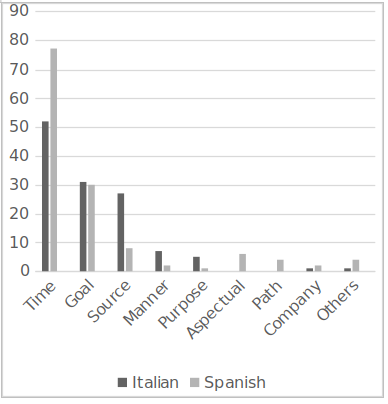
\includegraphics[scale=0.40]{../figures/nishida_f1.png}}
\quad
\ffigbox[\FBwidth]{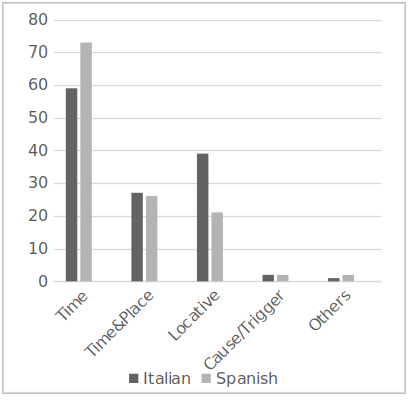
\includegraphics[scale=0.40]{../figures/nishida_f2.png}}{\caption{Graph of \textit{morire/}\\\textit{morir} VS preverbal adverbials}
    \label{fig:nishida:2}}
\end{floatrow}
\end{figure}

\begin{figure}

\begin{floatrow}
\ffigbox[\FBwidth]{\caption{Graph of \textit{cadere/caer}\\ VS preverbal adverbials}\label{fig:nishida:3}}{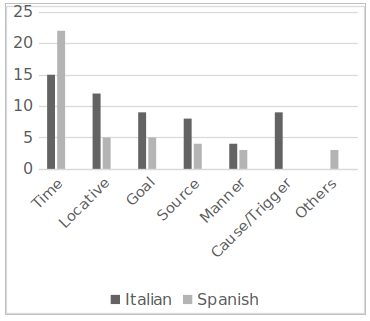
\includegraphics[scale=0.40]{../figures/nishida_f3.png}}
    \qquad
\ffigbox[\FBwidth]{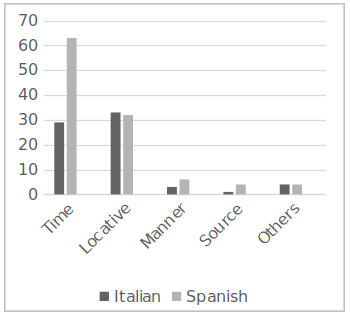
\includegraphics[scale=0.40]{../figures/nishida_f4.png}}{\caption{Graph of \textit{comparire/aparecer}\\ VS preverbal adverbials }
    \label{fig:nishida:4}}
\end{floatrow}
\end{figure}

\newpage
As is evident in \figref{fig:nishida:1}--\figref{fig:nishida:4}, the most dominant semantic category of preverbal adverbials used across all pairs of verbs is Time, conforming to the predictions made by the proponents of the s\textsc{top}.

With respect to spatial adverbials, our results show that across the four pairs of verbs, five main semantic categories of preverbal adverbials are found: \textsc{Goal, Source, Path, Locative}, and \textsc{Time\&Space}. We will take each pair of verbs and closely examine whether their co-occurring spatial adverbials fit in the definition of the s\textsc{top} or not. First, note that \citet{lahousse2007implicit} fine-tunes the definition of the s\textsc{top} as the ``the scene at which the event takes place'' \ref{ex:nishida:8}, when explaining why directional XPs may not serve as s\textsc{top}s  in French. However, this definition would result in different spatial categories for the four pair of verbs under consideration. Note that all pairs of verbs denote telic events that yield some type of change as they come to their final point. In the traditional theory of aspect these predicates are defined as achievements, which have an inherent endpoint (cf. \citealt{smith1997}); in the more recent theory of lexical semantics (cf. \citealt{beavers2011affectedness}) they are the so-called verbs of quantized change (i.e., verbs entailing a specific final goal on a scale of change), as pointed out by B\&C (\citeyear{bentley2018silent}). So, from the spatial point of view, the s\textsc{top} (or SoP) corresponds to the location at which quantized change occurs.  

For \textit{arrivare/llegar}, such a location is what is characterized as \textsc{Goal} above (and also by B\&C \citeyear{bentley2018silent}). Indeed, \textsc{Goal}, which is defined as the thematic argument of \textit{arrivare/llegar}, is the most frequently used semantic category of adverbials after \textsc{Time}, as shown in \figref{fig:nishida:1} and illustrated in \ref{ex:nishida:9} below.  


\begin{exe} % declares the example environment
    \ex\label{ex:nishida:9} 
\textsc{Goal} \quad \textbf{A los mercados de Murcia} llegan los higos chumbos. (Sp.; press)

 \glt `At the markets of Murcia arrive prickly pears.'\\
\end{exe}

However, as is also very notable in \figref{fig:nishida:1}, we found a few tokens of Source, particularly in the Italian corpus, as illustrated in \ref{ex:nishida:10} below. Moreover, though much fewer, there were some tokens of \textsc{Path} in the Spanish corpus, as shown in the bracketed sentence in \ref{ex:nishida:11}. 

\begin{exe} % declares the example environment
    \ex\label{ex:nishida:10} 
 \textsc{Source} \quad	\textbf{Dalla Germania} arrivano notizie pesanti come macigni. 
 (It.; fiction)
\glt `\textbf{From Germany} arrives news as heavy as boulders.'
\end{exe}

\begin{exe} % declares the example environment
    \ex\label{ex:nishida:11} 
\textsc{Path} \quad  Irún es la frontera ferroviaria que registra un mayor número de pasajeros procedentes del exterior {\dots};
[\textbf{por la estación de las Fuentes de Oñoro} llegan los	provinentes de Portugal.] (Sp.; non-fiction)

 \glt `Irún is the railway border that records a great number of passengers coming from   outside {\dots}; [\textbf{through the station of las Fuentes de Oñoro} arrive those coming 	from Portugal.'\\
\end{exe}

Clearly, neither the \textsc{Source} nor \textsc{Path} adverbial would qualify as a s\textsc{top} because they correspond to the phase of the event prior to the scene at which the event is complete. When faced with these sentences, we have two alternative positions available for analysis. One is to postulate that the  \textsc{Source} or \textsc{Path} adverbial is not serving as a preverbal topic, but there is actually a covert s\textsc{top} in \ref{ex:nishida:10} or \ref{ex:nishida:11} licensing subject inversion. The second position is to accept that  \textsc{Source} or \textsc{Path}  serves as a topical frame for the sentence to follow just as \textsc{Goal} does. We argue for the second position on some empirical grounds. 

First, the covert s\textsc{top} analysis runs into a problem right away judging from what Lahousse herself says. In characterizing the s\textsc{top}s, \citep[9]{lahousse2007implicit} cautions that not all preverbal locative or temporal adverbials and connectives in VS sentences are serving as s\textsc{top}s and licensing inversion. For instance, she claims that deictic or anaphoric locatives like `from there', `a bit further', `here', etc., as well as temporals like `now', `today', `finally', `soon', `already', `immediately', `afterwards', etc., do not function as s\textsc{top}s because they do not directly provide spatio-temporal locations for inversion sentences. She postulates that when this type of adverbial appears in the preverbal position it is followed by a covert s\textsc{top}. However, neither the Source in \ref{ex:nishida:10} nor the \textsc{Path} adverbial in \ref{ex:nishida:11}, fits the description of those that cannot serve as s\textsc{top}s, which weakens an analysis that assumes the presence of a covert preverbal s\textsc{top} triggering subject inversion in \ref{ex:nishida:10} or \ref{ex:nishida:11}. 

Second, the preverbal \textsc{Source} or \textsc{Path} XPs, as in \ref{ex:nishida:10} and \ref{ex:nishida:11}, are no different from the preverbal \textsc{Goal} in \ref{ex:nishida:9} above, in that it is presupposed (i.e., identifiable because of its unique referent). Therefore, each one is a topical element that serves as a frame within which the predication holds. As mentioned above, when depicting an event of arrival, \textsc{Source} or \textsc{Path} correspond to a phase prior to the final phase \textsc{Goal}, where change of location is complete. Depending on the message the speaker/writer wishes to convey, these phases may constitute a critical aspect of the event of arrival for the speaker/writer from the communicative point of view; therefore, they may use \textsc{Source} or \textsc{Path} as a framework within which the sentence is to be asserted or negated. Note that for the arrival of objects like news, orders, letters, messages, etc., \textsc{Source} is a natural and valid choice for the topical adverbial, even more so than \textsc{Goal}. Equally, \textsc{Path} (i.e., port of entry) can effectively frame the arrival of foreign travelers originating from different countries. For this reason, we hold that the preverbal topical adverbial for \textit{arrivare/llegar} need not be universally restricted to \textsc{Goal} across the board, as claimed in previous studies.

B\&C's (\citeyear{bentley2018silent}) claim that the covert preverbal adverbial (i.e., SoP) for arrival events must be \textsc{Goal} is also empirically too narrowly defined. In order to support their claim, they argue that VS sentences with \textit{arrivare} cannot have a \textsc{Goal} PP postverbally because there is already a covert \textsc{Goal} PP preverbally. However, we found obvious counterexample to this argument, as shown in \ref{ex:nishida:12} for both languages. 


\begin{exe} % declares the example environment
    \ex\label{ex:nishida:12} 
    \begin{xlist}
\ex\label{ex:nishida:12a}  Arrivano \textbf{in redazione} centinaia di telefonate di ascoltatori.	(It.; fiction)
\glt `There arrive \textbf{to the editorial office} hundreds of listeners' calls.' 

\ex\label{ex:nishida:12b} Aun así, todavía llegaron miles de españoles \textbf{a Dríus}.  (Sp.; press) 
\glt `Even so, there still arrived thousands of Spaniards \textbf{in Dríus}.'  
    \end{xlist}
\end{exe}

With respect to \textit{morire/morir}, the spatial adverbial that fits the definition of the s\textsc{top} is what we have categorized as \textsc{Locative} and \textsc{Time\&Space}, the latter of which is illustrated in \ref{ex:nishida:13} below. As shown in \figref{fig:nishida:2}, these are two semantic categories of which we have found most tokens besides \textsc{Time}; there was no other category with a notable number of tokens found.

\begin{exe}
    \ex\label{ex:nishida:13}
    \textsc{Time\&Space} \quad	\textbf{Nell'assalto} sono morte almeno dieci persone. (It.; press)
    \glt `I\textbf{n the assault} at least ten people died.'
\end{exe}

The next pair of verbs is \textit{cadere/caer}, which also denote change of location. Although B\&C (\citeyear{bentley2018silent}) do not discuss \textit{cadere}, it critically differs from \textit{arrivare} in that with \textit{cadere} change of location may have two directional orientations: \textsc{Goal} and \textsc{Source}. Additionally, the event of falling may be depicted without a particular directional orientation. If so, \textsc{Locative} will be the choice of the spatial location where quantized change occurs. All three of these semantic categories may serve equally well as preverbal topics with \textit{cadere/caer}, as is evident in \figref{fig:nishida:3}, and illustrated in \ref{ex:nishida:14}--\ref{ex:nishida:16} below. 

\begin{exe}
    \ex\label{ex:nishida:14}
    \textsc{Goal} \quad	Così dicendo, rovesciò il sacchetto e [\textbf{sul tavolo}] caddero due calze nuove, 						identiche a quelle rovinate].	(It.; fiction)
    
    \glt `Saying that, he turned the little bag upside down and [\textbf{on the table}] fell two new socks identical to the ruined ones.'   
\end{exe}

\begin{exe}
    \ex\label{ex:nishida:15}
    \textsc{Source} \quad	[\textbf{Del cielo}] caen dos diablos.	(Sp.; fiction)
    \glt `[\textbf{From the heavens}] fall two devils.'
\end{exe}

\begin{exe}
    \ex\label{ex:nishida:16}
    \textsc{Locative} \quad La meteorologia impazzisce: [\textbf{a Tokyo}] cadono pezzi di ghiaccio grossi come meloni] (It; miscellanea)
    \glt `Meteorology goes mad: [\textbf{in Tokyo}] fall pieces of ice as large as melons].'    
\end{exe}

The verbs of appearance \textit{comparire/aparaecer} denote change of state; therefore the spatial preverbal adverbial that qualifies as a s\textsc{top} for this pair of verbs is \textsc{Locative}. As shown in \figref{fig:nishida:4}, this is the category with the most tokens after \textsc{Time}. Nevertheless, we also found some tokens of Source adverbials which do not qualify as s\textsc{top}s, as illustrated in \ref{ex:nishida:17}. 



\begin{exe}
    \ex\label{ex:nishida:17}
    
    \textsc{Source} \quad	{\dots} \textbf{desde todos los rincones del claustro} aparecieron hasta 75
    flautistas que dedicaron al gran maestro Rampal la versión más ennoblecida {\dots}\
    (Sp.; press) 
    \glt `{\dots} \textbf{from all corners of the cloister} appeared as many as 75 	flutists who dedicated to the great master Rampal the most distinguished 	version {\dots}'  
\end{exe}

By the same reasoning used above for preverbal Source adverbials with \textit{arrivare/llegar}, we also assume that the \textsc{Source} adverbial in \ref{ex:nishida:17} serves as a topical element licensing subject inversion. Note that in this depiction of an act of surprise, the Source adverbial constitutes an integral aspect of the event, which makes it a valid choice to serve as a framework for the event in which an amazing number of flutists emerged to play ``Happy Birthday'' for the word-renowned flutist. 

Browsing through all graphs, we also see preverbal adverbials that cannot be defined as s\textsc{top}s because they have nothing to do with Space or Time. Among those, two categories stand out: \textsc{Cause/Trigger} and \textsc{Manner}, as illustrated in \ref{ex:nishida:18} and \ref{ex:nishida:19}, respectively.  

\begin{exe}
    \ex\label{ex:nishida:18}
    
    \textsc{Cause/Trigger} \quad	\textbf{Con i nuovi media} cadono le dicotomie tradizionali. 
    (It.; non-fiction)
    \glt `\textbf{With the (advent of the) new media} fall (out) the traditional 										dichotomies.'
\end{exe}

\begin{exe}
    \ex\label{ex:nishida:19}
    
    \textsc{Manner} \quad \textbf{Por docenas} aparecieron las personas que insistían en que también habían visto hadas. (Sp.; non-fiction)
    \glt `\textbf{By the dozens} appeared persons who would insist that they had also seen fairies.'     
\end{exe}

Are the  \textsc{Cause/Trigger} and  \textsc{Manner} adverbials in these sentences serving as topical elements to license subject inversion? We postulate that they do. In both cases, the preverbal XP is presupposed because the author of these sentences can assume that its referent is known to the reader. Moreover, looking at the metaphorical nature of the falling event depicted in \ref{ex:nishida:18}, it may be more relevant to frame the event from the perspective of what  caused/triggered the fall (out) rather than  \textsc{where} (or  \textsc{when}) it occurred. Likewise, the event of appearance in \ref{ex:nishida:19} can be framed by how it occurred, if that is what the writer intended to convey and contextually appropriate. Therefore, we hold that the  \textsc{Cause/Trigger} in \ref{ex:nishida:18} or the  \textsc{Manner} adverbial in \ref{ex:nishida:19} should serve as a valid framework within which the veracity of the event depicted can be evaluated. 	 

Through a qualitative analysis of our corpus data, we have evaluated whether the preverbal topical elements for VS unaccusative sentences must meet the definition of the s\textsc{top}. First, we have found that the s\textsc{top} (or SoP), as defined as the spatio-temporal location in which quantized change takes place, indeed constitutes the most common type of topical framework for subject inversion constructions in Italian and Spanish. However, we have demonstrated that the topical element in question is not restricted to what has been defined as the s\textsc{top} by its proponents. In fact, it extends to other semantic categories corresponding to more diverse circumstantial phases/aspects of the event involved, in accordance with the perspective that the speaker/writer wishes to adopt to frame it. We have provided examples in which non-\textsc{Goal} spatial categories like \textsc{Source} and \textsc{Path}, serve as the topical adverbial for \textit{arrivare/llegar} as well as examples in which non-spatio-temporal categories like \textsc{Cause/Trigger} and \textsc{Manner} license subject inversion.

Although an exhaustive analysis of all tokens is beyond the scope of the present study, our finding so far suggest that there are more cases supporting the argument that the preverbal element to license subject inversion in Romance languages goes beyond what is defined as the s\textsc{top}, SoP, or \textsc{loc} in previous research.\footnote{\citet[27]{casielles2004syntax} observes that ``in Spanish almost any category can be placed in the sentence-initial position if it is considered to be topical: PP, AdjP, VP, QP, CP, etc.'', suggesting that sentence-initial phrases do not necessarily refer to discourse entities. }

Before closing this section, we address two issues not pertaining to adverbials. As mentioned above, \citet[2, original italics]{cornish2005cross} claims that the role of inversion sentences is ``to \textit{present} a referent which is discourse new within the framework of a locative or temporal context''. Furthermore, he characterizes the verb used in these sentences as ``a locative or existential non predicating verb whose inherent semantics corresponds or is reduced to this type of denotation''. This last view is held by many others, who postulate that verbs used in presentational sentences are informationally ``light'' (cf. \citealt{suner1982}; \citealt{birner1994information}; \citealt{zubizarreta1998}, \textit{inter alia}; for a refutation of both claims, on the other hand, see \citealt{marandin2010subject}). With respect to the first issue, our corpus data reveal that the subject referent is most typically discourse new, as shown in \ref{ex:nishida:1} and many other examples seen above. However, being discourse new is not a necessary condition, since a well-known object/person or a unique object needing no prior introduction may appear as the subject of a presentational sentence (cf. \textit{Esta noche llegan los Reyes} `This evening arrive the King and the Queen'). As for the second issue, we also agree with \citet{marandin2010subject} that it is not quite accurate to state that \textit{morire/morir} in \ref{ex:nishida:1}, for instance, are used merely as existential verbs and do not denote a dying event, while the opposite holds for \ref{ex:nishida:2}. Nonetheless, as we look at SV sentences more in detail below and the contrast between VS and SV sentences becomes clearer, the two constructions appear to underscore different aspects of an event. VS sentences foreground the ``emergence'' of the subject referent, where the verb specifies how the referent is made visible (or audible) by arrival/death/fall/appearance, etc. However, we hold that this ``presentational'' sense does not stem from the inherent meaning of the verb but is associated with the VS construction itself. The fact that VS sentences rarely have any other adverbial following the subject (mean length: 0.25 word for Italian; 0.26 word for Spanish) corroborates that the introduction of the subject referent into the discourse is the primary role of VS sentences.

\subsection{SV sentences and postverbal adverbials}

As shown in \tabref{tab:nishida:6} our corpus data reveals that SV sentences most commonly contain 1 or 2 postverbal adverbials. In contrast to VS sentences, SV sentences without postverbal adverbials are less frequent, especially in Spanish.  

\begin{table}
    \begin{tabular}{lrr}\lsptoprule
     & Italian & Spanish\\\midrule
     Zero & 43 (19\%) & 22 (5\%)\\
   One & 121 (53\%) & 261 (53\%)\\
   Two & 60 (26\%) & 169 (34\%)\\
   Three & 6 (3\%) & 33 (7\%)\\
   Four & & 4 (1\%)\\
   & 230 (Means 1.1) & 489 (Means 1.4)\\
   \lspbottomrule
    \end{tabular}
    \caption{SV sentences: number of postverbal adverbials}
    \label{tab:nishida:6}
\end{table}

\figref{fig:nishida:5}--\figref{fig:nishida:8} give the breakdown of the types of postverbal adverbials occurring with each pair of  verbs.


\begin{figure}

\begin{floatrow}
\ffigbox[\FBwidth]{\caption{Graph of \textit{arrivare/llegar} SV\\ postverbal adverbials}\label{fig:nishida:5}}{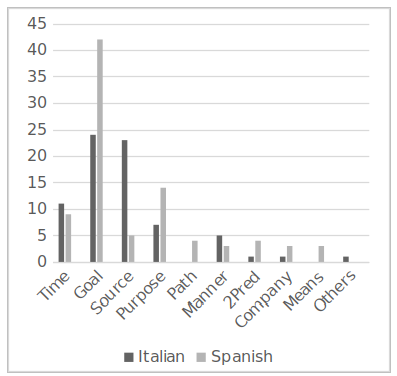
\includegraphics[scale=0.40]{../figures/nishida_f5.png}}
\quad
\ffigbox[\FBwidth]{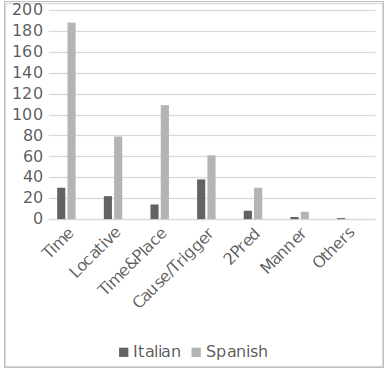
\includegraphics[scale=0.40]{../figures/nishida_f6.png}}{\caption{Graph of \textit{morire/morir} SV\\ postverbal adverbials }
    \label{fig:nishida:6}}
\end{floatrow}
\end{figure}

\begin{figure}

\begin{floatrow}
\ffigbox[\FBwidth]{\caption{Graph of \textit{cadere/caer} SV\\ postverbal}\label{fig:nishida:7}}{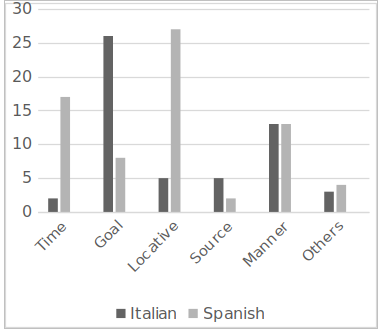
\includegraphics[scale=0.40]{../figures/nishida_f7.png}}
\quad
\ffigbox[\FBwidth]{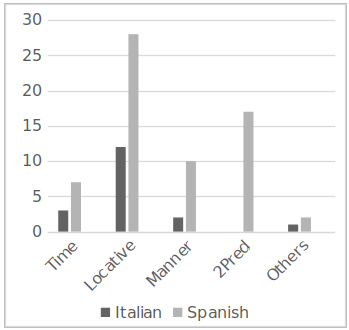
\includegraphics[scale=0.40]{../figures/nishida_f8.png}}{\caption{Graph of \textit{comparire/aparecer} SV\\ postverbal adverbials }
    \label{fig:nishida:8}}
\end{floatrow}
\end{figure}

\newpage

Postverbal adverbials in SV sentences differ crucially from preverbal adverbials in VS sentences in that Time, which was the predominant category for all pairs of verbs (cf. \figref{fig:nishida:1}--\figref{fig:nishida:4}), occurs in much smaller numbers over all. In its place, a new set of categories such as \textsc{Purpose} (with `arriving'), \textsc{Cause/Trigger} (with `dying'), \textsc{Manner} (with `falling' and `appearing'), and \textsc{2Pred} (with `dying' and `appearing' in Spanish) are integrated into SV sentences along with various spatio-temporal categories, as exemplified in \ref{ex:nishida:20}--\ref{ex:nishida:23} below.

\begin{exe}
    \ex\label{ex:nishida:20}
    
   Giovani e vecchi arrivano [\textbf{da tutta Italia}] [\textbf{per ricostruire l'edificio distrutto dalle ruspe del Comune}] (It.; press)
    \glt `Young and old people arrive [\textbf{from all Italy}] [\textbf{to rebuild the building destroyed by the 		city's excavators}].'   
\end{exe}

\begin{exe}
    \ex\label{ex:nishida:21}
    
   Un milione e ottocentomila bambini muoiono [\textbf{ogni anno}] [\textbf{per malattie causate 					dall'acqua inquinata}]. (It.; press)
    \glt `One million eight hundred thousand children die [\textbf{every year}] [\textbf{from diseases caused by 		polluted water}].'  
\end{exe}

\begin{exe}
    \ex\label{ex:nishida:22}
    
   Le carte caddero [\textbf{per terra}] [\textbf{con un fruscio di fiocchi nevosi}]. (It.; fiction)
    \glt `The papers fell [\textbf{to the floor}] [\textbf{with a snowflake-like rustling}].'  
\end{exe}


\begin{exe}
    \ex\label{ex:nishida:23}
    
   Mesalina y Catalina aparecen [\textbf{en escena}] [\textbf{vestidas de señoras de la limpieza}], [\textbf{con un cubo y una escoba cada una}]. (Sp.; fiction)
    \glt `Mesalina and Catalina emerge [\textbf{in the scene}] [\textbf{dressed as cleaning ladies}], [\textbf{with a bucket and a broom each}].'
\end{exe}

\citet{teixeira2016locative} argues that, unlike in English, postverbal adverbials are always focal in Romance languages. As evident in the above examples, since they are part of the focus, these adverbials may be grammatically heavy and richer in details than preverbal adverbials serving as topical elements in VS sentences. In fact, PPs containing an infinitival clause like in \ref{ex:nishida:24} below or \ref{ex:nishida:20} above, appear as postverbal adverbials, an option not found for preverval adverbials.  

\begin{exe}
    \ex\label{ex:nishida:24}
    
   Una mujer con orden de protección muere [\textbf{tras ser atropellada tres veces por su	esposo}]. (Sp.; press)
    \glt `A woman with a protection order die after being driven over three times by her husband.'
\end{exe}

In essence, postverbal adverbials in SV sentences are describing not only \textsc{when} and \textsc{where} but also \textsc{how} and \textsc{why} an event comes about. From these facts, it is clear that the SV sentences are not simply used to introduce a subject referent to the scene of the communication; rather, they are used to depict a new event unfolding with circumstantial details. It is also important to note that the event is reported without being framed by a topical (i.e. presupposed) element, as is clear in \ref{ex:nishida:2} above. Therefore, the event depicted in an SV sentence is perceived as emerging ``out-of-the-blue'', and for this reason, it is particularly suited for a headline and the first sentence of a news piece, as shown in \ref{ex:nishida:25}, where there is no presupposed prior information concerning the event reported. 


\begin{exe}
    \ex\label{ex:nishida:25}
  Dos inmigrantes africanos mueren en Alemania en un atentado del PKK. BONN. 	(Corresponsal.) – Dos inmigrantes africanos murieron ayer en la ciudad de Ulm, en el	sur de Alemania, en un incendio presumiblemente provocado. (Sp.; press) 
    \glt `Two African immigrants die in Germany in an assault of the PKK. BONN. 	(Correspondent.) – Two African immigrants died yesterday in the city of Ulm, in the south of Germany, in a fire presumably provoked.'
\end{exe}

However, as the results of the quantitative analysis reported in \ref{sec:nishida:2} have shown, SV sentences are not only restricted to newspaper's headlines, but they may also appear in different genres as well as in the middle of a passage, as illustrated in \ref{ex:nishida:2a} above. 

\section{Conclusion}\label{sec:nishida:5}

In this paper we have shown that Italian and Spanish VS and SV unaccusative sentences in SF contexts are not free variants but represent two distinct constructions each associated with a particular discourse function. VS sentences (\textit{aka} locative inversion) are used to report a new event highlighting the (dis)appearance of the subject referent within a framework of a typically – but not exclusively – presupposed spatio-temporal location, which may be explicitly represented by a preverbal adverbial, or anaphorically or deictically recoverable. SV sentences also report a new event; nonetheless, they highlight its process aspect by giving rich circumstantial details. Critically, the event reporting does not involve framing by a topical element. Although we have limited our study to VS and SV sentences with unaccusatives, a similar contrast can be predicted to exist between VS and SV sentences with unergatives. That the same verb may be used in two syntactic frames depending on what aspect of the event is (de)emphasized has a non-trivial consequence for the lexicon-syntax interface involving intransitive verbs in general. 

\section*{Corpora}

\textit{Corpus di italiano scritto} (CORIS/CODIS, \url{http://corpora.dslo.unibo.it/coris_ita.html})
\textit{Corpus de referencia del español actual} (CREA, \url{http://corpus.rea.es/creanet.html})

\section*{Acknowledgements}

We would like to thank two anonymous reviewers for their insightful comments and suggestions, and Adrián R. Riccelli for conducting the statistics. Also, we are very grateful to Chad Lewis and his assistant Camila Lívio for their help with the editorial process, and to Laurie Modrey for checking the English translation of all our data and Elisenda Grigsby for proofreading the text.

\printbibliography[heading=subbibliography,notkeyword=this]

\end{document}